\documentclass[11pt]{article}

\usepackage[margin=1in]{geometry}
\usepackage{amsmath, amssymb}
\usepackage{microtype}
\usepackage{xcolor}
\usepackage{hyperref}
\usepackage{enumitem}
\usepackage{parskip}
\usepackage{tikz}
\usetikzlibrary{decorations.markings, arrows.meta}

\tikzset{
  arr/.style={decoration={markings, mark=at position 0.62 with {\arrow{Stealth}}}, postaction={decorate}},
  arrc/.style={decoration={markings, mark=at position 0.5 with {\arrow{Stealth}}}, postaction={decorate}}
}

\hypersetup{
  colorlinks=true,
  linkcolor=blue!60!black,
  urlcolor=blue!60!black
}

\newcommand{\R}{\mathbb{R}}
\newcommand{\C}{\mathbb{C}}
\newcommand{\HH}{\mathbb{H}}
\newcommand{\OO}{\mathbb{O}}
\newcommand{\Z}{\mathbb{Z}}

\title{\textbf{Quaternions and Octonions, from the Coordinate Plane}}
\author{}
\date{}

\begin{document}
\maketitle

\vspace{-2em}

\section*{Start where you are: the coordinate plane}

You know the coordinate plane. A point is a pair of numbers
$(x, y)$. You go $x$ steps right and $y$ steps up. That's it.
The plane is just $\R^2$: pairs of real numbers.

You can already \emph{add} points like vectors:
\[
(3, 2) + (1, 4) = (4, 6) .
\]
Component-wise. No surprises.

But here's the question that sets up everything else:

\begin{quote}
  Can we also \emph{multiply} two points and get a third point, in a
  way that's actually useful?
\end{quote}

For real numbers on a line, multiplication is obvious: $3 \times 2 =
6$. What does $(3,2) \times (1,4)$ even mean? You could try
multiplying component-wise --- $(3 \cdot 1, 2 \cdot 4) = (3, 8)$ ---
but that turns out to be boring and not useful for anything. We want
a multiplication rule that means something.

\section*{The 2D answer: complex numbers}

Here is the cleverest possible multiplication on the plane. Pick a
special point and call it $i$. We'll put $i$ at $(0, 1)$ ---
one step up the vertical axis.

Define one rule:
\[
i \cdot i \;=\; -1 .
\]

That single rule, plus ``multiplication should behave like normal
multiplication otherwise'' (distributive, associative, commutative),
forces \emph{every other product}. A general point $(a, b)$ on the
plane gets written as $a + b\,i$, and then you just multiply out:
\[
(a + b\,i)(c + d\,i)
\;=\; ac + ad\,i + bc\,i + bd\,i^2
\;=\; (ac - bd) + (ad + bc)\,i .
\]

So in coordinates:
\[
(a, b) \cdot (c, d) \;=\; (ac - bd, \; ad + bc) .
\]

That's it. That's all complex numbers are: \emph{the coordinate plane
with that one multiplication rule}. The letter ``$i$'' is just the
name of the point $(0, 1)$. There is nothing imaginary about it.

\subsection*{Why this rule is magic}

Try multiplying any point by $i$:
\[
i \cdot (a, b) \;=\; (0, 1) \cdot (a, b) \;=\; (-b, \; a) .
\]

Look at what happened: $(a, b)$ became $(-b, a)$. That is exactly a
$90^{\circ}$ counter-clockwise rotation about the origin.

Multiplying by $i$ \emph{rotates the plane by $90^{\circ}$}.

More generally, multiplying by any complex number scales the plane
and rotates it by a fixed angle. Complex multiplication \emph{is}
the language of $2$D rotation-and-scaling. This is why complex
numbers show up in electrical engineering, signal processing,
quantum mechanics --- anywhere you need to rotate things.

\textbf{The summary so far:}
\begin{itemize}[leftmargin=*, itemsep=2pt]
  \item Real numbers $\R$: a $1$D line.
  \item Complex numbers $\C$: the $2$D plane, with a multiplication
        that captures rotation.
\end{itemize}

That extra structure --- being able to multiply --- is what makes
$\C$ way more useful than just ``pairs of numbers.''

\section*{Hamilton's question (the obvious next move)}

If $\C$ is the plane with a useful multiplication, can we do the same
thing in $3$D? Can we put a useful multiplication on
$\R^3$ --- triples $(x, y, z)$ --- that captures rotations in
$3$D space?

This question consumed William Rowan Hamilton, an Irish
mathematician, for over a decade. He kept trying. He kept failing.
His sons used to ask him at breakfast, ``Well, Papa, can you
multiply triples?'' and he would say, sadly, ``No, I can only add and
subtract them.''

The reason he was stuck: \emph{it is impossible}. There is no useful
multiplication on $\R^3$. You can prove it.

\section*{The breakthrough: use 4 dimensions, not 3}

On October 16, 1843, Hamilton was walking with his wife along the
Royal Canal in Dublin, on his way to a meeting at the Royal Irish
Academy. He realised --- in a flash, the way these things happen
--- that he didn't need three dimensions. He needed \emph{four}.

He took his pocket-knife and carved the formula into the stone of
Brougham Bridge:
\[
i^2 \;=\; j^2 \;=\; k^2 \;=\; i\,j\,k \;=\; -1 .
\]

The carving is gone, but there is a plaque on the bridge today
commemorating the moment. This was the birth of \textbf{quaternions}.

\section*{What quaternions are}

A quaternion is a point in $4$D space:
\[
q \;=\; a + b\,i + c\,j + d\,k ,
\]
where $a, b, c, d$ are real numbers and $i, j, k$ are three special
``unit'' directions, each perpendicular to the others and to the
``real'' direction.

The set of all quaternions is called $\HH$, after Hamilton.

The multiplication rule is everything in
\[
i^2 = j^2 = k^2 = -1, \qquad
ij = k, \quad jk = i, \quad ki = j .
\]

(Same cyclic pattern as the right-hand rule.) And here is the
twist:
\[
ji = -k, \quad kj = -i, \quad ik = -j .
\]

\textbf{Order matters.} $ij \neq ji$. Quaternions are
\emph{non-commutative}. This is the first new thing.

\subsection*{The bargain: you trade commutativity for an extra dimension}

\begin{itemize}[leftmargin=*, itemsep=2pt]
  \item Real numbers ($1$D): you can multiply, and $ab = ba$.
  \item Complex numbers ($2$D): you can multiply, and $ab = ba$.
  \item Quaternions ($4$D): you can multiply, but $ab \neq ba$
        in general.
\end{itemize}

Every time you double the dimension, you get a useful multiplication
rule, but you pay for it by giving up a property you took for
granted.

\section*{What quaternions are good for}

Just as multiplying by a complex number rotates the plane,
multiplying by a quaternion rotates $3$D space. Specifically:
sandwich a $3$D vector $v$ between a quaternion $q$ and its
``conjugate'' $q^{-1}$:
\[
v \;\mapsto\; q\,v\,q^{-1} .
\]
The result is $v$ rotated. The quaternion $q$ encodes the axis and
angle of rotation.

This is not a toy. Quaternions are how:
\begin{itemize}[leftmargin=*, itemsep=2pt]
  \item Video games and $3$D animation software smoothly rotate
        objects without ``gimbal lock'' (the failure mode of just
        using three angles).
  \item Aerospace and robotics track orientation.
  \item Physicists describe the spin of electrons (via the closely
        related \emph{Pauli matrices}).
\end{itemize}

If you have ever rotated a camera in Unity or Unreal or Blender,
quaternions did the work.

\section*{Doing the trick again: octonions}

We doubled the dimension from $1$ to $2$ (real $\to$ complex) and
got rotations of the plane. We doubled from $2$ to $4$ (complex
$\to$ quaternion) and got rotations of $3$D space. There is a
recipe --- the \emph{Cayley--Dickson construction} --- for doing
this doubling mechanically. So: what happens if we double again?

You get an $8$-dimensional algebra called the \textbf{octonions},
written $\OO$. Discovered by John Graves in late $1843$ (just two
months after Hamilton's quaternions) and independently by Arthur
Cayley in $1845$.

An octonion is a point in $8$D space, with one real direction and
seven ``imaginary'' directions $e_1, e_2, \dots, e_7$. They each
square to $-1$, they each anticommute with the others, and the
products $e_i e_j$ follow a specific rule.

But what is the rule? Writing out all $7 \times 7 = 49$ products in
a table is awful. There is a much better way to present them: the
\emph{Fano plane}.

\subsection*{The Fano plane: octonion multiplication in one picture}

\begin{center}
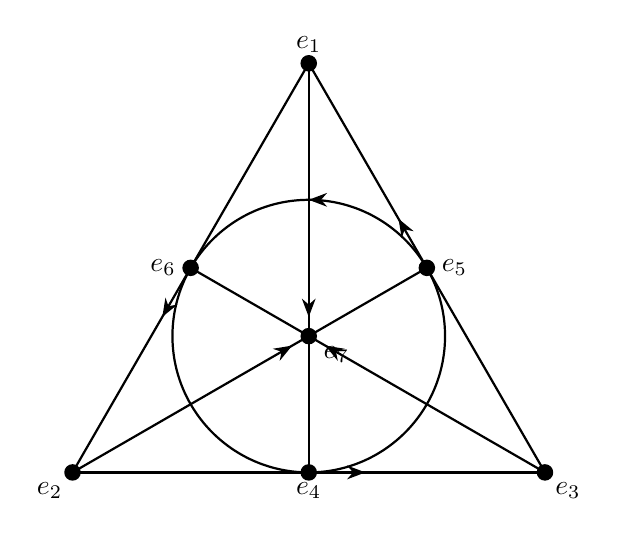
\begin{tikzpicture}[scale=3, line width=0.8pt]
  \coordinate (e1) at (0, 1.732);
  \coordinate (e2) at (-1, 0);
  \coordinate (e3) at (1, 0);
  \coordinate (e4) at (0, 0);
  \coordinate (e5) at (0.5, 0.866);
  \coordinate (e6) at (-0.5, 0.866);
  \coordinate (e7) at (0, 0.577);

  % Sides of the triangle (oriented)
  \draw[arr] (e2) -- (e3);  % bottom:  e2 -> e4 -> e3
  \draw[arr] (e3) -- (e1);  % right:   e3 -> e5 -> e1
  \draw[arr] (e1) -- (e2);  % left:    e1 -> e6 -> e2

  % Medians (oriented)
  \draw[arr] (e1) -- (e4);  % e1 -> e7 -> e4
  \draw[arr] (e2) -- (e5);  % e2 -> e7 -> e5
  \draw[arr] (e3) -- (e6);  % e3 -> e7 -> e6

  % Inscribed circle (oriented counter-clockwise: e4 -> e5 -> e6 -> e4)
  \draw[arrc] (e7) ++(-90:0.577) arc[start angle=-90, end angle=270, radius=0.577];

  % Points
  \foreach \p in {e1,e2,e3,e4,e5,e6,e7} {
    \fill (\p) circle (0.035);
  }

  % Labels
  \node[above]      at (e1) {$e_1$};
  \node[below left] at (e2) {$e_2$};
  \node[below right]at (e3) {$e_3$};
  \node[below]      at (e4) {$e_4$};
  \node[right]      at (e5) {\,$e_5$};
  \node[left]       at (e6) {$e_6$\,};
  \node[below right]at (e7) {\,$e_7$};
\end{tikzpicture}
\end{center}

\textbf{What you are looking at.} The Fano plane is the smallest
projective plane. It has exactly:
\begin{itemize}[leftmargin=*, itemsep=2pt]
  \item $7$ points (the $7$ imaginary units $e_1, \dots, e_7$);
  \item $7$ lines, each containing exactly $3$ points;
  \item the property that any two points lie on a unique line.
\end{itemize}
Six of the lines are drawn straight; the seventh is the circle
through the three edge-midpoints. ``Line'' here means
``line of the projective plane'' --- the circle is geometrically a
circle but combinatorially a line.

\textbf{How to read it as a multiplication table.} Each line carries
an orientation (the arrows). If a line points
$e_a \to e_b \to e_c \to e_a$ cyclically, then
\[
  e_a\, e_b \;=\; e_c, \qquad
  e_b\, e_c \;=\; e_a, \qquad
  e_c\, e_a \;=\; e_b ,
\]
and going \emph{against} the arrow flips the sign:
\[
  e_b\, e_a \;=\; -e_c, \quad
  e_c\, e_b \;=\; -e_a, \quad
  e_a\, e_c \;=\; -e_b .
\]
Together with $e_i^2 = -1$, that is the entire octonion multiplication.

\textbf{The seven lines spelled out.} For our labelling above:

\begin{center}
\begin{tabular}{l l l}
\textbf{Line} & \textbf{Oriented triple} & \textbf{Products} \\
\hline
bottom side       & $e_2 \to e_4 \to e_3 \to e_2$ & $e_2 e_4 = e_3,\; e_4 e_3 = e_2,\; e_3 e_2 = e_4$ \\
right side        & $e_3 \to e_5 \to e_1 \to e_3$ & $e_3 e_5 = e_1,\; e_5 e_1 = e_3,\; e_1 e_3 = e_5$ \\
left side         & $e_1 \to e_6 \to e_2 \to e_1$ & $e_1 e_6 = e_2,\; e_6 e_2 = e_1,\; e_2 e_1 = e_6$ \\
median from $e_1$ & $e_1 \to e_7 \to e_4 \to e_1$ & $e_1 e_7 = e_4,\; e_7 e_4 = e_1,\; e_4 e_1 = e_7$ \\
median from $e_2$ & $e_2 \to e_7 \to e_5 \to e_2$ & $e_2 e_7 = e_5,\; e_7 e_5 = e_2,\; e_5 e_2 = e_7$ \\
median from $e_3$ & $e_3 \to e_7 \to e_6 \to e_3$ & $e_3 e_7 = e_6,\; e_7 e_6 = e_3,\; e_6 e_3 = e_7$ \\
inscribed circle  & $e_4 \to e_5 \to e_6 \to e_4$ & $e_4 e_5 = e_6,\; e_5 e_6 = e_4,\; e_6 e_4 = e_5$ \\
\end{tabular}
\end{center}

\textbf{Worked example.} To compute $e_3 \cdot e_5$: find the unique
line through $e_3$ and $e_5$ --- the right side of the triangle.
The orientation is $e_3 \to e_5 \to e_1$, and the arrow goes from
$e_3$ \emph{to} $e_5$, so
\[
  e_3 e_5 \;=\; e_1 .
\]
To compute $e_5 \cdot e_3$ instead: same line, against the arrow, so
$e_5 e_3 = -e_1$.

\subsection*{Why the Fano plane?}

There is something marvellous in the fact that octonion
multiplication is encoded in a tiny combinatorial object. The Fano
plane is one of the most studied objects in finite geometry: it is
the projective plane $\mathrm{PG}(2, \mathbb{F}_2)$ over the field
with two elements. The same picture shows up in the
theory of error-correcting codes (the binary $[7,4]$ Hamming code),
in the structure of the simple group $\mathrm{PSL}_2(\mathbb{F}_7)$,
and now in the multiplication table of the octonions. It is the
smallest projective plane that exists at all --- and it carries
exactly enough structure to define an $8$-dimensional division
algebra. That coincidence is part of why the octonions feel
miraculous.

\subsection*{The next bargain}

\begin{itemize}[leftmargin=*, itemsep=2pt]
  \item Real numbers $\R$ ($1$D): commutative, associative.
  \item Complex numbers $\C$ ($2$D): commutative, associative.
  \item Quaternions $\HH$ ($4$D): \emph{not commutative}, but still
        associative.
  \item Octonions $\OO$ ($8$D): not commutative \emph{and not
        associative}.
\end{itemize}

\emph{Associative} means $(a \cdot b) \cdot c$ equals $a \cdot (b
\cdot c)$ --- you can group the parentheses however you want.
With octonions, this fails: $(a b) c$ and $a (b c)$ can be different
octonions. Almost every algebraic tool you have ever used quietly
assumed associativity. Without it, normal calculation becomes
treacherous.

\section*{Why stop at 8?}

Try doubling again. You can. The result is the $16$-dimensional
``sedenions.'' But now the bargain has changed: the sedenions have
\emph{zero divisors}. You can find two nonzero sedenions whose
product is zero. That means you can't divide, and the structure
breaks badly. Past dimension $8$, the doubling trick stops giving
you something useful.

This is a theorem, not a fashion:

\begin{quote}
  \textbf{Hurwitz's theorem (1898).} The only \emph{normed division
  algebras} over $\R$ have dimensions $1$, $2$, $4$, or $8$.
\end{quote}

In plain terms: real numbers, complex numbers, quaternions and
octonions are the \emph{only} ways to put a well-behaved
multiplication on $\R^n$. There is no $5$D or $7$D version. There
is no $16$D version. The four are the whole list.

Even more remarkable: a much harder result (Frobenius, with later
work by Bott, Milnor, Kervaire and Adams) connects these dimensions
to deep topological facts about spheres. The numbers $1, 2, 4, 8$
are not a coincidence; they're the same dimensions in which the
$n$-sphere can be ``parallelised'' (combed without a cowlick). The
fact that there are exactly four normed division algebras is
secretly the same fact as the fact that you can comb hair flat on
$S^1$, $S^3$ and $S^7$ but not on any other sphere.

\section*{The cheat sheet}

\begin{center}
\begin{tabular}{lcl}
\textbf{Algebra} & \textbf{Dim.} & \textbf{What you give up} \\
\hline
$\R$ (real numbers)         & $1$ & nothing \\
$\C$ (complex numbers)      & $2$ & ordering (no ``which is bigger'') \\
$\HH$ (quaternions)         & $4$ & commutativity ($ab \neq ba$) \\
$\OO$ (octonions)           & $8$ & associativity ($(ab)c \neq a(bc)$) \\
\end{tabular}
\end{center}

\section*{Why octonions are still interesting if you can't even multiply with parentheses}

Octonions are weird, and for a long time they were considered a
curiosity. But over the last fifty years they have shown up in
several deep places:

\begin{itemize}[leftmargin=*, itemsep=2pt]
  \item The five \emph{exceptional Lie groups} ($G_2$, $F_4$,
        $E_6$, $E_7$, $E_8$) --- bizarre symmetry groups that have
        no infinite-family explanation --- are all built from the
        octonions. $G_2$ is literally the automorphism group of
        $\OO$.
  \item In particle physics, octonions show up in proposed
        descriptions of fundamental particles (the
        ``three generations'' of fermions match the $\OO$
        structure suspiciously well), and in string theory and
        $M$-theory, the special role of dimensions $10$ and $11$
        is closely tied to the octonions.
  \item In number theory and lattice theory, the densest known
        sphere packings in $8$ and $24$ dimensions ($E_8$ and the
        Leech lattice) are built using octonionic arithmetic.
\end{itemize}

So the joke is on us: the algebra that seemed least useful for
ordinary calculation turns out to underlie some of the most
exceptional and beautiful structures in mathematics.

\section*{Practical aside: can you use this in Vulkan?}

Vulkan is a graphics API. The question is fair: if quaternions
rotate $3$D space and octonions are the next step up, can a shader
or a graphics engine actually \emph{use} octonions for anything?

\subsection*{Quaternions: yes, everywhere}

Quaternions are the standard way to represent and compose rotations
in real-time graphics, and Vulkan is no exception. In practice:

\begin{itemize}[leftmargin=*, itemsep=2pt]
  \item You store a unit quaternion as a \texttt{vec4} on the CPU
        side and pass it to a shader as a uniform or vertex
        attribute. GLSL/SPIR-V has no native quaternion type, but
        you only need a handful of helper functions: quaternion
        multiplication, conjugate, and the rotation sandwich
        $v \mapsto q\,v\,q^{-1}$ (which simplifies for unit $q$).
  \item Skeletal animation systems store bone orientations as
        quaternions because they interpolate well: spherical linear
        interpolation (``slerp'') gives smooth, constant-speed
        rotation between two orientations, with no gimbal lock and
        no normalisation drift problems that Euler angles would have.
  \item Cameras, IMU integration, and orientation tracking all use
        quaternion arithmetic for the same reasons.
\end{itemize}

If you write a Vulkan renderer, you will end up writing or importing
a quaternion library. That is essentially mandatory.

\subsection*{Octonions: effectively no, and there is a real reason}

Octonions cannot replace quaternions for $3$D rotation, and there is
nowhere else in a standard graphics pipeline that they slot in. The
specific obstacles:

\begin{itemize}[leftmargin=*, itemsep=2pt]
  \item \textbf{Non-associativity wrecks composition.} The reason
        quaternions are useful is that composing two rotations is the
        same as multiplying their quaternions: rotate-by-$q_1$ then
        rotate-by-$q_2$ becomes rotate-by-$q_2 q_1$. Octonion
        multiplication is \emph{not} associative, so
        $(q_1 q_2) v (q_1 q_2)^{-1}$ is not the same as
        $q_1\bigl(q_2 v q_2^{-1}\bigr) q_1^{-1}$. You cannot ``stack''
        octonion rotations the way you do quaternion rotations,
        because the algebra refuses to cooperate.
  \item \textbf{Unit octonions are not a group.} Unit quaternions form
        the sphere $S^3$, which is a Lie group, which is exactly what
        rotations need. Unit octonions form $S^7$, which is famously
        \emph{not} a group --- it is a Moufang loop, a weaker
        structure. There is no group of $3$D rotations sitting inside
        the octonions.
  \item \textbf{$3$D space doesn't fit.} The natural geometric home
        of octonions is in dimensions $7$ and $8$ (where they
        actually do encode special rotations, via the exceptional
        groups $G_2$, $\mathrm{Spin}(7)$ and $\mathrm{Spin}(8)$).
        Graphics pipelines work in dimension $3$, where the
        octonionic structure is, simply, the wrong tool.
\end{itemize}

\subsection*{So where might octonions plausibly appear?}

Honest answer: nowhere in the mainline rendering pipeline. The
places they do appear are research-flavoured and far from a typical
Vulkan workload:

\begin{itemize}[leftmargin=*, itemsep=2pt]
  \item \emph{Octonionic and Clifford neural networks.} Some
        research groups have built networks whose weights live in
        $\HH$ or $\OO$, motivated by signal-processing problems with
        natural multi-channel structure. These can in principle run
        on a GPU, but not via Vulkan's graphics path --- they look
        like ordinary tensor workloads to a compute backend.
  \item \emph{Geometric algebra / Clifford algebra renderers.}
        A small community uses geometric algebra
        ($\mathrm{Cl}_{3,0}$, $\mathrm{Cl}_{3,1}$, etc.) as a unifying
        framework for graphics math. These algebras are cousins of
        the quaternions and octonions, but the actual workhorses are
        the Clifford algebras, not $\OO$ itself.
  \item \emph{Exotic research demos.} You can write a shader that
        evaluates an octonion fractal (the analogue of the Mandelbrot
        set in $\OO$), or that visualises subsets of
        $7$-dimensional space using octonionic structure. These are
        beautiful and useless, in the best mathematical tradition.
\end{itemize}

\textbf{Bottom line.} In Vulkan, quaternions are essential; octonions
have no native role in $3$D rendering. The reason is structural ---
non-associativity --- not a missing library.

\subsection*{OK fine --- here is how to actually put octonions in Vulkan}

You can absolutely put octonions in a Vulkan shader. The issue is not
``can you'', it is ``what do you do with them.'' Octonions are 8
floats and a multiplication rule; GPUs eat 8 floats for breakfast.
Here are the genuinely viable things to do:

\paragraph{1. Octonion fractals (the fun answer).}
Just as the Mandelbrot set lives in $\C$ and quaternion Julia sets
live in $\HH$, you can iterate $z \mapsto z^2 + c$ in $\OO$ and get
\emph{octonion fractals}. Since the result lives in $8$D, you take a
$3$D slice (fix five of the eight coordinates) and render it as a
volumetric or signed-distance object in a fragment shader. This is
the closest thing to a ``real'' Vulkan use of octonions, and people
do render these.

\paragraph{2. Octonion neural networks (compute shader workloads).}
Some research uses octonion-valued weights for signal-processing
tasks with natural $7$- or $8$-channel structure (multi-spectral
imagery, certain audio problems). Vulkan compute shaders are a
perfectly reasonable backend; you're not using the graphics pipeline,
but you are using Vulkan.

\paragraph{3. Procedural noise / high-dimensional sampling.}
The seven imaginary units give you a $7$D direction space with rich
algebraic structure. You can use it as the substrate for a procedural
noise function with built-in symmetries you would not get from
$\R^7$.

\paragraph{The GLSL skeleton.} Define an octonion as a \texttt{vec4 +
vec4} pair (real part plus seven imaginary components, packed
naturally on $16$-byte boundaries):

\begin{verbatim}
struct Oct {
    float r;       // real part
    float e[7];    // e_1 ... e_7
};

// Multiplication using the Fano-plane rules.
// Each pair (e_i, e_j) is on exactly one line; the line tells you
// which e_k you get and with what sign. The 21 sign rules below
// come directly from the seven oriented triples in the Fano plane.
Oct omul(Oct a, Oct b) {
    Oct c;
    c.r = a.r*b.r - a.e[0]*b.e[0] - a.e[1]*b.e[1] - a.e[2]*b.e[2]
                  - a.e[3]*b.e[3] - a.e[4]*b.e[4] - a.e[5]*b.e[5]
                  - a.e[6]*b.e[6];
    // imaginary parts: scalar*imag + imag*scalar + cross-products
    // following the Fano lines. (Expand the 7 lines into 7*3 = 21
    // pairwise products, with anticommutativity giving the rest.)
    // ... (~50 lines of straight-line arithmetic)
    return c;
}
\end{verbatim}

The expansion of the cross-products is mechanical from the table of
seven Fano lines given earlier. There is no branching, no recursion,
no loops --- just a fixed pile of multiply-adds, which is exactly
what a GPU executes fastest.

\paragraph{Octonion fractal fragment shader, in outline.}
\begin{verbatim}
// for each pixel:
Oct c = octFromUV(uv);              // pick c from screen + sliders
Oct z = octZero();
for (int i = 0; i < MAX_ITER; ++i) {
    z = oadd(omul(z, z), c);
    if (onorm2(z) > 4.0) break;
}
// shade based on i (escape time) or use a distance estimator
\end{verbatim}

\paragraph{What this won't do.} It will not make your rotations
better, replace your quaternion library, or give you any new graphics
primitive. What it \emph{will} do is let you render objects nobody
else has, because the slice of $\OO$ you choose to project is yours
to pick. If ``octonions in Vulkan'' is the project, the octonion
fractal viewer is the actual thing to build.

\section*{Recap, in one breath}

The coordinate plane is just $\R^2$ until you give it a multiplication
rule; then it becomes $\C$, and that rule is exactly $2$D rotation.
Doubling the dimension gives $\HH$, which encodes $3$D rotation, at
the cost of $ab \neq ba$. Doubling once more gives $\OO$, which
gives up associativity too. Doubling beyond that breaks. The four
algebras $\R, \C, \HH, \OO$ are the complete list of well-behaved
multiplications you can put on $\R^n$, and the same four dimensions
$1, 2, 4, 8$ show up in topology, Lie theory and physics in ways
nobody fully understands.

\section*{Further reading}

\begin{itemize}[leftmargin=*, itemsep=2pt]
  \item John Baez, ``The Octonions,'' \emph{Bulletin of the AMS}
        \textbf{39} (2002), 145--205. The standard friendly
        survey; readable by undergraduates, deep enough for
        researchers.
  \item John Stillwell, \emph{Naive Lie Theory}, Springer, $2008$.
        Beautiful book that builds up to quaternions and beyond from
        the coordinate plane.
  \item John H.\ Conway and Derek A.\ Smith, \emph{On Quaternions
        and Octonions}, A.\ K.\ Peters, $2003$. Short, authoritative,
        readable.
  \item Marcus du Sautoy, \emph{Finding Moonshine}, Fourth Estate,
        $2008$. Includes a chapter on quaternions and the bridge
        story.
\end{itemize}

\end{document}
